\documentclass[english,preprint]{elsarticle}

% --- Page layout ---
\usepackage{geometry}
\geometry{a4paper, margin=0.7in}

\usepackage[T1]{fontenc}
\usepackage[utf8]{inputenc}
\usepackage{lmodern}
\usepackage{microtype}
\usepackage{amsmath,amssymb}
\usepackage{booktabs}
\usepackage{tabularx}
\usepackage{longtable}
\usepackage{array}
\usepackage{graphicx}
\usepackage{placeins}
\usepackage{enumitem}
\usepackage{url}
\usepackage{hyperref}
\usepackage{xcolor}
\usepackage{siunitx}
\usepackage{caption}
\usepackage{xspace}
\usepackage{rotating}

\journal{Results in Engineering}
\biboptions{sort&compress}
\hypersetup{colorlinks=true,linkcolor=blue,citecolor=blue,urlcolor=blue}
\sisetup{detect-all}

\newcolumntype{Y}{>{\raggedright\arraybackslash}X}
\newcommand{\CAD}{\textsc{CAD}\xspace}
\newcommand{\indicator}[1]{\mathbb{I}\!\left[#1\right]}

\begin{document}

\begin{frontmatter}

\title{Clinical-Architectural Debt: Process-Aware Maintenance Prioritization for Distributed Electronic Health Record Systems}

\author[ilam]{Mohammad Tanhaei\corref{cor1}}
\ead{m.tanhaei@ilam.ac.ir}
\ead[url]{https://orcid.org/0000-0001-5089-3917}
\cortext[cor1]{Corresponding author}
\address[ilam]{Department of Engineering, Ilam University, Ilam, Iran}

\begin{abstract}
Distributed Electronic Health Record (EHR) systems increasingly rely on service-oriented and microservice-based architectures while supporting clinical workflows whose safety relevance varies substantially across pathways. Existing technical-debt and architectural-debt approaches can identify structural degradation, but they usually prioritize debt using software-centric proxies such as coupling, instability, complexity, change-proneness, or test gaps. In safety-relevant healthcare software, such proxies may be incomplete when used alone because the engineering priority of a component also depends on the clinical pathways it supports and the criticality assigned to those pathways.

This paper introduces \emph{Clinical-Architectural Debt} (\CAD), a process-aware architectural-debt metric and analysis pipeline for distributed EHR systems. \CAD combines component-level structural fragility with pathway frequency, expert-assessed clinical criticality, and trace-to-component mappings derived from runtime observability data. The method is intended to support engineering decisions, specifically refactoring prioritization and architectural maintenance; it is not a clinical decision-support tool and does not certify patient safety.

In this simulation-only working version, we evaluate \CAD on a deterministic synthetic BioArc-like architecture using generated activity counts, simulated trace-link coverage, configured pathway criticality, and 120 injected architecture-level defects distributed across 12 relevant components. The study compares \CAD against static-fragility, frequency-only, and unweighted process-aware baselines using ranking and retrieval metrics. The results are interpreted as preliminary evidence of engineering prioritization effectiveness in the evaluated setting rather than proof of clinical safety impact. The main contribution is a specified and empirically evaluated formulation of process-aware architectural debt, together with reproducibility-oriented materials for maintenance prioritization in safety-relevant healthcare software.
\end{abstract}

\begin{keyword}
architectural technical debt \sep healthcare software \sep electronic health records \sep process mining \sep microservices \sep empirical software engineering
\end{keyword}

\end{frontmatter}

\begin{center}
\fbox{\parbox{0.94\textwidth}{\small\textbf{Simulation-only working version.}
All values in the empirical section of this file were generated by the
public synthetic calibration code at
\url{https://github.com/tanhaei/CAD}. They are temporary reproducibility
placeholders and are not a substitute for the independently verified outputs
of the original BioArc study.}}
\end{center}

\section{Introduction}\label{sec:introduction}

Healthcare software is moving toward distributed, service-oriented, and microservice-based architectures to improve scalability, interoperability, modular deployment, and organizational autonomy. The movement is visible both in general microservice research and in healthcare interoperability initiatives, especially HL7 FHIR and SMART-on-FHIR ecosystems \cite{Newman2015Microservices,Dragoni2017Microservices,Soldani2018PainsGains,Taibi2017Microservices,FHIR2026,Mandel2016SMART}. These architectural choices are attractive for EHR vendors and hospital information systems, but they also create a difficult maintenance problem: failures may no longer be localized to a single module. A clinical action such as medication ordering can traverse authentication, patient-identity, medication, allergy, drug--drug interaction, audit, billing, and notification services.

Technical debt was originally introduced as a metaphor for expedient design and implementation decisions whose long-term cost is paid later \cite{Cunningham1992WyCash,Kruchten2012TechnicalDebt,Li2015TechnicalDebt}. Later work distinguished code-level debt from architectural technical debt, where design decisions, dependency structures, and architectural decay create high maintenance cost and defect propagation risk \cite{Alves2016TechnicalDebt,Rios2018TertiaryStudy,Verdecchia2021Landscape,Martini2015ATD,Xiao2016ArchitecturalDebt,Soliman2021DesignDecisions,Verdecchia2021Theory}. Existing debt-management techniques are valuable, but they tend to emphasize software structure and development cost. In clinical software, however, two components with similar structural debt can have different safety relevance: a moderately coupled component in a chemotherapy workflow can be more urgent than a highly coupled archival component used only in non-critical reporting.

The core hypothesis of this work is that architectural-debt prioritization in EHR systems should not be based only on software structure. A structurally fragile component becomes more urgent when it is repeatedly executed within clinically important pathways. Conversely, a component with severe structural debt may be less urgent if it is isolated from safety-relevant workflows and is covered by adequate regression tests. \CAD operationalizes this distinction by combining architectural fragility with pathway exposure and clinical criticality.

Process mining provides methods for discovering and analyzing real processes from event logs \cite{VanderAalst2016Book,VanderAalst2012Manifesto}. In healthcare, it has been used to analyze patient trajectories, guideline deviations, care-flow complexity, and operational bottlenecks \cite{Rojas2016Healthcare,MunozGama2022Healthcare,DeRoock2022Perspective}. Yet most healthcare process-mining studies focus on clinical or organizational improvement rather than software architecture. Conversely, most architectural-debt studies focus on source-code and dependency structures rather than clinical workflow risk. The gap is therefore not merely bibliographic; it is methodological.

This article proposes \CAD, a process-aware architectural-debt formulation for distributed EHR systems. \CAD combines: (i) component fragility derived from structural and historical software indicators; (ii) clinical pathway frequency mined from event logs; (iii) pathway criticality elicited from clinical experts or risk models; and (iv) trace-to-component mappings derived from distributed tracing. The intended output is not a clinical diagnosis or medical recommendation. It is an engineering prioritization signal for architectural maintenance.

This study is organized around the following research questions:
\begin{description}[style=nextline,leftmargin=1.2cm,labelwidth=1cm]
  \item[\textbf{RQ1}] Does \CAD rank components containing injected architecture-level defects higher than software-only, usage-only, and unweighted process-aware baselines?
  \item[\textbf{RQ2}] What is the marginal contribution of clinical criticality weighting beyond process frequency and structural fragility?
  \item[\textbf{RQ3}] How robust are \CAD rankings to the removal of individual \CAD components, changes in scoring parameters, pathway-frequency thresholds, clinical-criticality scores, and trace-completeness assumptions?
  \item[\textbf{RQ4}] What is the computational overhead of computing \CAD for the evaluated event-log volume and trace-linking configuration?
\end{description}

The contributions of this paper are:
\begin{enumerate}
  \item A formal process-aware architectural-debt metric that combines component fragility, clinical pathway frequency, clinical criticality, and trace-derived component exposure.
  \item An analysis pipeline that operationalizes \CAD from event logs, distributed traces, architectural dependency data, and expert-rated pathway criticality.
  \item A controlled empirical case study comparing \CAD with static-fragility, frequency-only, and unweighted process-aware baselines, accompanied by reported trace coverage, confidence intervals, effect-size estimates, ablation results, and runtime-scalability measurements.
\end{enumerate}

The remainder of the paper is organized as follows. Section~\ref{sec:related} positions the work against architectural debt, healthcare process mining, and automated testing. Section~\ref{sec:model} defines the \CAD metric. Section~\ref{sec:pipeline} describes the analysis pipeline. Section~\ref{sec:evaluation} reports the empirical study design, ranking results, ablation results, and runtime measurements. Section~\ref{sec:discussion} discusses implications and potential applications. Section~\ref{sec:threats} discusses threats to validity. Section~\ref{sec:replication} describes the replication materials and the constraints governing access to the operational data. Section~\ref{sec:conclusion} concludes.

\section{Related Work}\label{sec:related}

\subsection{Technical debt and architectural technical debt}

Technical-debt research has matured from metaphorical descriptions to systematic management frameworks \cite{Cunningham1992WyCash,Kruchten2012TechnicalDebt,Li2015TechnicalDebt}. Systematic mapping and review studies show that debt management includes identification, measurement, prioritization, monitoring, repayment, and communication activities \cite{Alves2016TechnicalDebt,Rios2018TertiaryStudy,Lenarduzzi2021Prioritization}. Architectural technical debt is particularly difficult because it is often distributed across dependency structures, architectural decisions, team boundaries, and long-lived evolution patterns \cite{Martini2015ATD,Xiao2016ArchitecturalDebt,Soliman2021DesignDecisions,Verdecchia2021Theory}. \CAD builds on this body of work but changes the prioritization objective: a component is not only expensive to maintain; it can be clinically risky if it mediates high-criticality pathways.

\subsection{Microservices and EHR interoperability}

Microservices offer independently deployable services, fine-grained APIs, decentralized data management, and technology heterogeneity \cite{Newman2015Microservices,Dragoni2017Microservices,Soldani2018PainsGains,Taibi2017Microservices}. These features can support healthcare interoperability, but they also increase the testing and observability burden. In EHR ecosystems, FHIR and SMART-on-FHIR support standardized exchange and app integration \cite{FHIR2026,Mandel2016SMART}. However, interoperability does not eliminate architecture risk. A standardized API can still be part of a fragile, highly coupled, or poorly tested pathway.

\subsection{Process mining in healthcare}

Process mining discovers process models, checks conformance, and analyzes variants from event logs \cite{VanderAalst2016Book,VanderAalst2012Manifesto}. Healthcare process mining faces special challenges: patient heterogeneity, multi-disciplinary workflows, missing or noisy events, privacy constraints, and high variability of cases \cite{Rojas2016Healthcare,MunozGama2022Healthcare,DeRoock2022Perspective}. \CAD uses process mining differently from most clinical-flow studies. The process model is not the final object of analysis; it becomes a weighting mechanism for software architecture.

\subsection{Clinical safety, medication workflows, and decision-support failures}

Medication-related workflows are a canonical example of why software failures cannot be treated as ordinary enterprise defects. Computerized physician order entry can reduce serious medication errors when implemented with appropriate workflow support \cite{Bates1998CPOE}, but CPOE systems can also facilitate new error modes \cite{Koppel2005CPOE}. Clinical decision-support systems can improve practice under specific design conditions \cite{Kawamoto2005CDS}, but malfunctioning or misconfigured decision support can create patient-safety risks \cite{Wright2016Malfunctions}. Adverse-drug-event studies further motivate the need to treat medication and alerting workflows as high-criticality pathways \cite{Bates1995ADE}. \CAD does not solve clinical safety; it offers a software-engineering mechanism for ensuring that high-risk software paths are not deprioritized merely because their code metrics appear acceptable.

\subsection{Automated test generation and regression-test selection}

Automated testing research includes unit-test generation, REST API test generation, and service-oriented testing \cite{Fraser2011EvoSuite,Arcuri2018EvoMaster,Bozkurt2013SOATesting,Anand2013TestGeneration}. Regression-test selection and test-case prioritization have also been studied as cost-reduction techniques for evolving software systems \cite{Rothermel1996RTS,Yoo2012Regression,Elbaum2002Prioritization}. Traditional approaches prioritize tests using code coverage, changed entities, historical fault detection, execution cost, or requirements coverage. \CAD differs conceptually from these strategies by introducing a workflow- and criticality-aware weighting layer: a component's maintenance is prioritized not only because it is structurally fragile, but also because it participates in clinically important EHR pathways.

Table~\ref{tab:positioning} summarizes the distinction between \CAD and the adjacent research streams discussed above.

\begin{table}[htbp]
\caption{Positioning of \CAD relative to adjacent research streams.}
\label{tab:positioning}
\small
\begin{tabularx}{\textwidth}{@{}p{0.16\textwidth}Y Y Y@{}}
\toprule
\textbf{Stream} & \textbf{Typical object} & \textbf{Typical decision} & \textbf{Gap addressed by \CAD} \\
\midrule
Technical debt & Code smells, shortcuts, maintainability indicators & Refactoring and repayment prioritization & Adds pathway criticality and clinical frequency to debt ranking. \\
Architectural debt & Dependency structures, architectural decisions, change propagation & Architecture remediation & Weights architectural fragility by EHR execution paths and patient-safety relevance. \\
Healthcare process mining & Event logs, care pathways, variants, conformance & Clinical/operational improvement & Reuses process models to prioritize software architecture tasks. \\
Microservice testing & Service APIs, contracts, generated inputs, service interactions & Test generation and regression testing & Provides a foundation to constrain tests to clinically observed multi-hop paths. \\
\bottomrule
\end{tabularx}
\end{table}

\section{Formal Model}\label{sec:model}

\subsection{Architecture layer}

Let the distributed EHR architecture be represented as a directed weighted graph:
\begin{equation}
G=(C,E,W),
\label{eq:graph}
\end{equation}
where $C=\{C_1,\ldots,C_n\}$ is the set of deployable components, $E\subseteq C\times C$ is the set of observed or statically extracted dependencies, and $W:E\rightarrow \mathbb{R}^{+}$ assigns edge weights such as invocation frequency, payload size, synchronization strength, or change-propagation cost.

For component $C_j$, define structural fragility as a normalized score:
\begin{equation}
F(C_j)=\sum_{r=1}^{R}\alpha_r z_r(C_j),
\qquad
\sum_{r=1}^{R}\alpha_r=1,
\label{eq:fragility}
\end{equation}
where $z_r$ are normalized indicators such as instability, cyclic-dependency participation, recent defect density, change coupling, and test-gap ratio. The instability term can be computed using Martin's afferent/efferent coupling ratio:
\begin{equation}
\operatorname{Instability}(C_j)=
\frac{C_e(C_j)}{C_a(C_j)+C_e(C_j)+\epsilon}.
\label{eq:instability}
\end{equation}
The small $\epsilon$ avoids division by zero.

For the BioArc evaluation, the fragility vector comprised instability, cycle participation, recent defect density, change coupling, and test-gap ratio. Each indicator was normalized over the 45 evaluated components using 5th--95th percentile winsorized min--max scaling to $[0,1]$; values outside the percentile bounds were clipped before scaling. The fixed main-analysis weight vector was
\begin{equation}
\left(
\alpha_{\mathrm{instability}},
\alpha_{\mathrm{cycle}},
\alpha_{\mathrm{defect}},
\alpha_{\mathrm{change}},
\alpha_{\mathrm{test\mbox{-}gap}}
\right)
=
\left(0.20,0.15,0.25,0.20,0.20\right).
\label{eq:fragility-weights}
\end{equation}
The normalization rule and weights were fixed before the injected-defect labels were used for ranking assessment.

\subsection{Clinical process layer}

Let $A=\{a_1,\ldots,a_m\}$ be clinical activities recorded in EHR event logs. A pathway $P_i$ is a sequence or partially ordered trace:
\begin{equation}
P_i=\langle a_{i1},a_{i2},\ldots,a_{ik}\rangle.
\label{eq:pathway}
\end{equation}
The observed pathway frequency is:
\begin{equation}
f_i=\frac{N(P_i)}{\sum_{P_m\in\mathcal{P}}N(P_m)}.
\label{eq:frequency}
\end{equation}

The clinical criticality score $K(P_i)\in[0,1]$ may be elicited by a clinical panel, derived from incident-severity taxonomies, or modeled from risk categories. Because this variable can dominate the ranking, the study reports how criticality was elicited, who rated it, what rubric was used, and how disagreements were resolved. When more than two raters classify pathways into categorical risk bands, Fleiss' $\kappa$ is the appropriate agreement coefficient \cite{Fleiss1971}; Cohen's $\kappa$ is limited to the two-rater case \cite{Cohen1960}. Table~\ref{tab:criticality} gives the rubric used in the present study. If a deployment uses a different clinical-risk taxonomy, the score mapping is replaced and justified before \CAD scores are computed.

\begin{table}[htbp]
\caption{Clinical criticality rubric used for pathway scoring in the BioArc evaluation.}
\label{tab:criticality}
\small
\begin{tabularx}{\textwidth}{@{}p{0.11\textwidth}p{0.09\textwidth}Y p{0.12\textwidth}@{}}
\toprule
\textbf{Band} & \textbf{Score} & \textbf{Operational interpretation} & \textbf{Pathways in BioArc} \\
\midrule
Low & 0.25 & Administrative or documentation workflow with no immediate safety implication. & 4 \\
Moderate & 0.50 & Workflow delay or failure may affect care coordination but is unlikely to cause immediate harm. & 5 \\
High & 0.75 & Failure may affect diagnosis, medication, alerting, treatment timing, or handoff quality. & 3 \\
Critical & 1.00 & Failure may plausibly contribute to severe harm if not detected by downstream controls. & 2 \\
\bottomrule
\end{tabularx}
\end{table}

A frequency-only formulation can under-rank rare but high-criticality pathways. The primary analysis therefore used the normalized observed frequency $f_i$ in Equation~\eqref{eq:frequency} together with the criticality score $K(P_i)$. Robustness to pathway filtering was examined by increasing the rare-variant threshold from 0.5\% to 1.0\%, as reported in Table~\ref{tab:sensitivity}.

\subsection{Trace-to-component mapping}

Define a mapping function $\Phi:A\rightarrow 2^C$ that maps a clinical activity to the components executed during that activity. In practice, $\Phi$ is estimated from correlation IDs, distributed traces, logs, and API-gateway records. The architectural projection of pathway $P_i$ is:
\begin{equation}
G(P_i)=G\!\left[\bigcup_{a\in P_i}\Phi(a)\right],
\label{eq:projection}
\end{equation}
where $G[\cdot]$ denotes the induced subgraph.

Trace alignment is a major source of measurement error. The study therefore distinguishes three cases: complete mapping, partial mapping, and unmapped activity. Complete mapping means that all service hops for an activity are linked to a correlation identifier; partial mapping means that at least one hop is observed but the end-to-end trace is incomplete; unmapped activity means that no reliable runtime component can be assigned. The percentages of complete, partial, and unmapped activities are reported before \CAD scores are interpreted, because missing trace links can systematically understate the exposure of services that are weakly instrumented.

Table~\ref{tab:operational} summarizes the operational definitions used throughout the empirical study.

\begin{table}[htbp]
\caption{Operational definitions used in the BioArc evaluation.}
\label{tab:operational}
\small
\begin{tabularx}{\textwidth}{@{}p{0.18\textwidth}Y@{}}
\toprule
\textbf{Construct} & \textbf{Operational definition} \\
\midrule
Component & A deployable service or component represented in the architecture graph and ranked as one evaluation unit. \\
Dependency & A directed interaction encoded in $G$ from static architecture data or runtime observations, including API calls, message events, database access, or trace-derived service interactions. \\
Fragility & The weighted and normalized combination of instability, cycle participation, recent defect density, change coupling, and test-gap ratio defined in Equation~\eqref{eq:fragility}. \\
Clinical pathway & An event-log variant discovered with Inductive Miner after application of the pre-specified noise and rare-variant thresholds. \\
Criticality & The consensus score assigned by three clinical-informatics raters using the rubric in Table~\ref{tab:criticality}, with agreement quantified by Fleiss' $\kappa$. \\
Ground truth & A component-level relevance label indicating whether the component contained at least one injected architecture-level defect. \\
\bottomrule
\end{tabularx}
\end{table}

\subsection{Clinical-Architectural Debt}

The \CAD score for component $C_j$ is:
\begin{equation}
\operatorname{CAD}(C_j)=F(C_j)
\sum_{P_i\in\mathcal{P}_{\mathrm{active}}}
 f_i\,K(P_i)\,\indicator{C_j\in G(P_i)}.
\label{eq:cad}
\end{equation}
Equation~\eqref{eq:cad} defines the component-level score evaluated in this study. Edge-level and system-level aggregates are possible extensions, but they were not included in the reported empirical analysis.

\section{CAD Analysis Pipeline}\label{sec:pipeline}

The \CAD pipeline contains five stages.

\subsection{Stage 1: Event-log preparation}

The input event table contains a case identifier, activity label, timestamp, actor role, system action identifier, and optional severity or contextual fields. The operational logs were de-identified before analysis. The case-study filtering and process-discovery parameters are reported in Table~\ref{tab:setup}.

\subsection{Stage 2: Process discovery and variant extraction}

Pathway variants were discovered from the BioArc event log using Inductive Miner with a noise threshold of 0.8. Variants representing less than 0.5\% of total observed frequency were excluded from the primary pathway set. The resulting primary set contained 14 pathways. The effect of increasing the threshold to 1.0\% was evaluated in the sensitivity analysis.

\subsection{Stage 3: Distributed trace alignment}

Clinical activities were linked to runtime services using correlation identifiers, distributed traces, application logs, and API-gateway records. Each activity was classified as completely mapped, partially mapped, or unmapped according to the definitions in Section~\ref{sec:model}. Mapping coverage was measured before \CAD scores were computed.

\subsection{Stage 4: CAD scoring and ranking}

Components were scored using Equation~\eqref{eq:cad}. The scoring configuration comprised the fixed fragility weights, the four-level criticality rubric in Table~\ref{tab:criticality}, the pathway-filtering threshold, and the measured trace-linking coverage. Ranking effectiveness was evaluated using the measures defined in Section~\ref{sec:evaluation}.

\subsection{Stage 5: Engineering action}

The ranked list produced by Stage~4 supports engineering actions, specifically refactoring prioritization. Rather than serving as a clinical safety certification, \CAD provides a decision-support signal for software maintenance. Its purpose is to help engineering teams align remediation effort with components that are structurally fragile and highly exposed to safety-relevant clinical workflows. Any claim that \CAD reduces patient harm would require prospective operational evidence beyond the scope of this study.

\section{Empirical Evaluation on BioArc}\label{sec:evaluation}

For this simulation-only replication, we instantiated a synthetic BioArc-like distributed EHR architecture using the dimensions reported for BioArc \cite{BioArc2026}. The experiment assessed component-level prioritization against deterministic synthetic injected-defect labels; it did not evaluate patient outcomes, production incidents, or clinical safety.

\subsection{Research questions and study design}

The empirical study follows the four research questions introduced in Section~\ref{sec:introduction}. RQ1 evaluates whether \CAD improves ranking effectiveness over simpler baselines. RQ2 isolates the contribution of the clinical criticality term $K(P_i)$. RQ3 examines whether rankings remain stable when individual \CAD components are removed and when scoring parameters, pathway-frequency thresholds, clinical-criticality scores, and trace-completeness assumptions are perturbed. RQ4 measures runtime overhead. The unit of ranking is a deployable service or component, and the primary ground truth is a set of injected architecture-level defects.

All effectiveness values in Tables~\ref{tab:performance}--\ref{tab:sensitivity} are aggregated over 30 runs using seeds 42--71. In each run, pathway-level activity counts were resampled from a multinomial distribution and complete, partial, and unmapped trace-link states were independently resampled using the configured coverage probabilities; relevance labels were held fixed. The number of components labeled relevant was 12 of 45. The 95\% confidence intervals were obtained by a run-level bias-corrected and accelerated (BCa) bootstrap with 10,000 resamples.

\subsection{Experimental setup and architecture}

The evaluated BioArc deployment comprised 45 deployable services and components. External requests passed through Nginx, HAProxy, and the authentication layer before reaching the BioArc core and domain services. MariaDB stored structured clinical and audit data, Redis supported sessions, queues, and temporary state, and ClickHouse supported passive analytics. Figure~\ref{fig:bioarc-overview} presents the simplified architecture used to explain the data sources required by \CAD. Detailed service-integration and observability views are provided in Appendix~\ref{app:architecture}, Figures~\ref{fig:appendix-service} and~\ref{fig:appendix-observability}.

\begin{figure}[htbp]
\centering
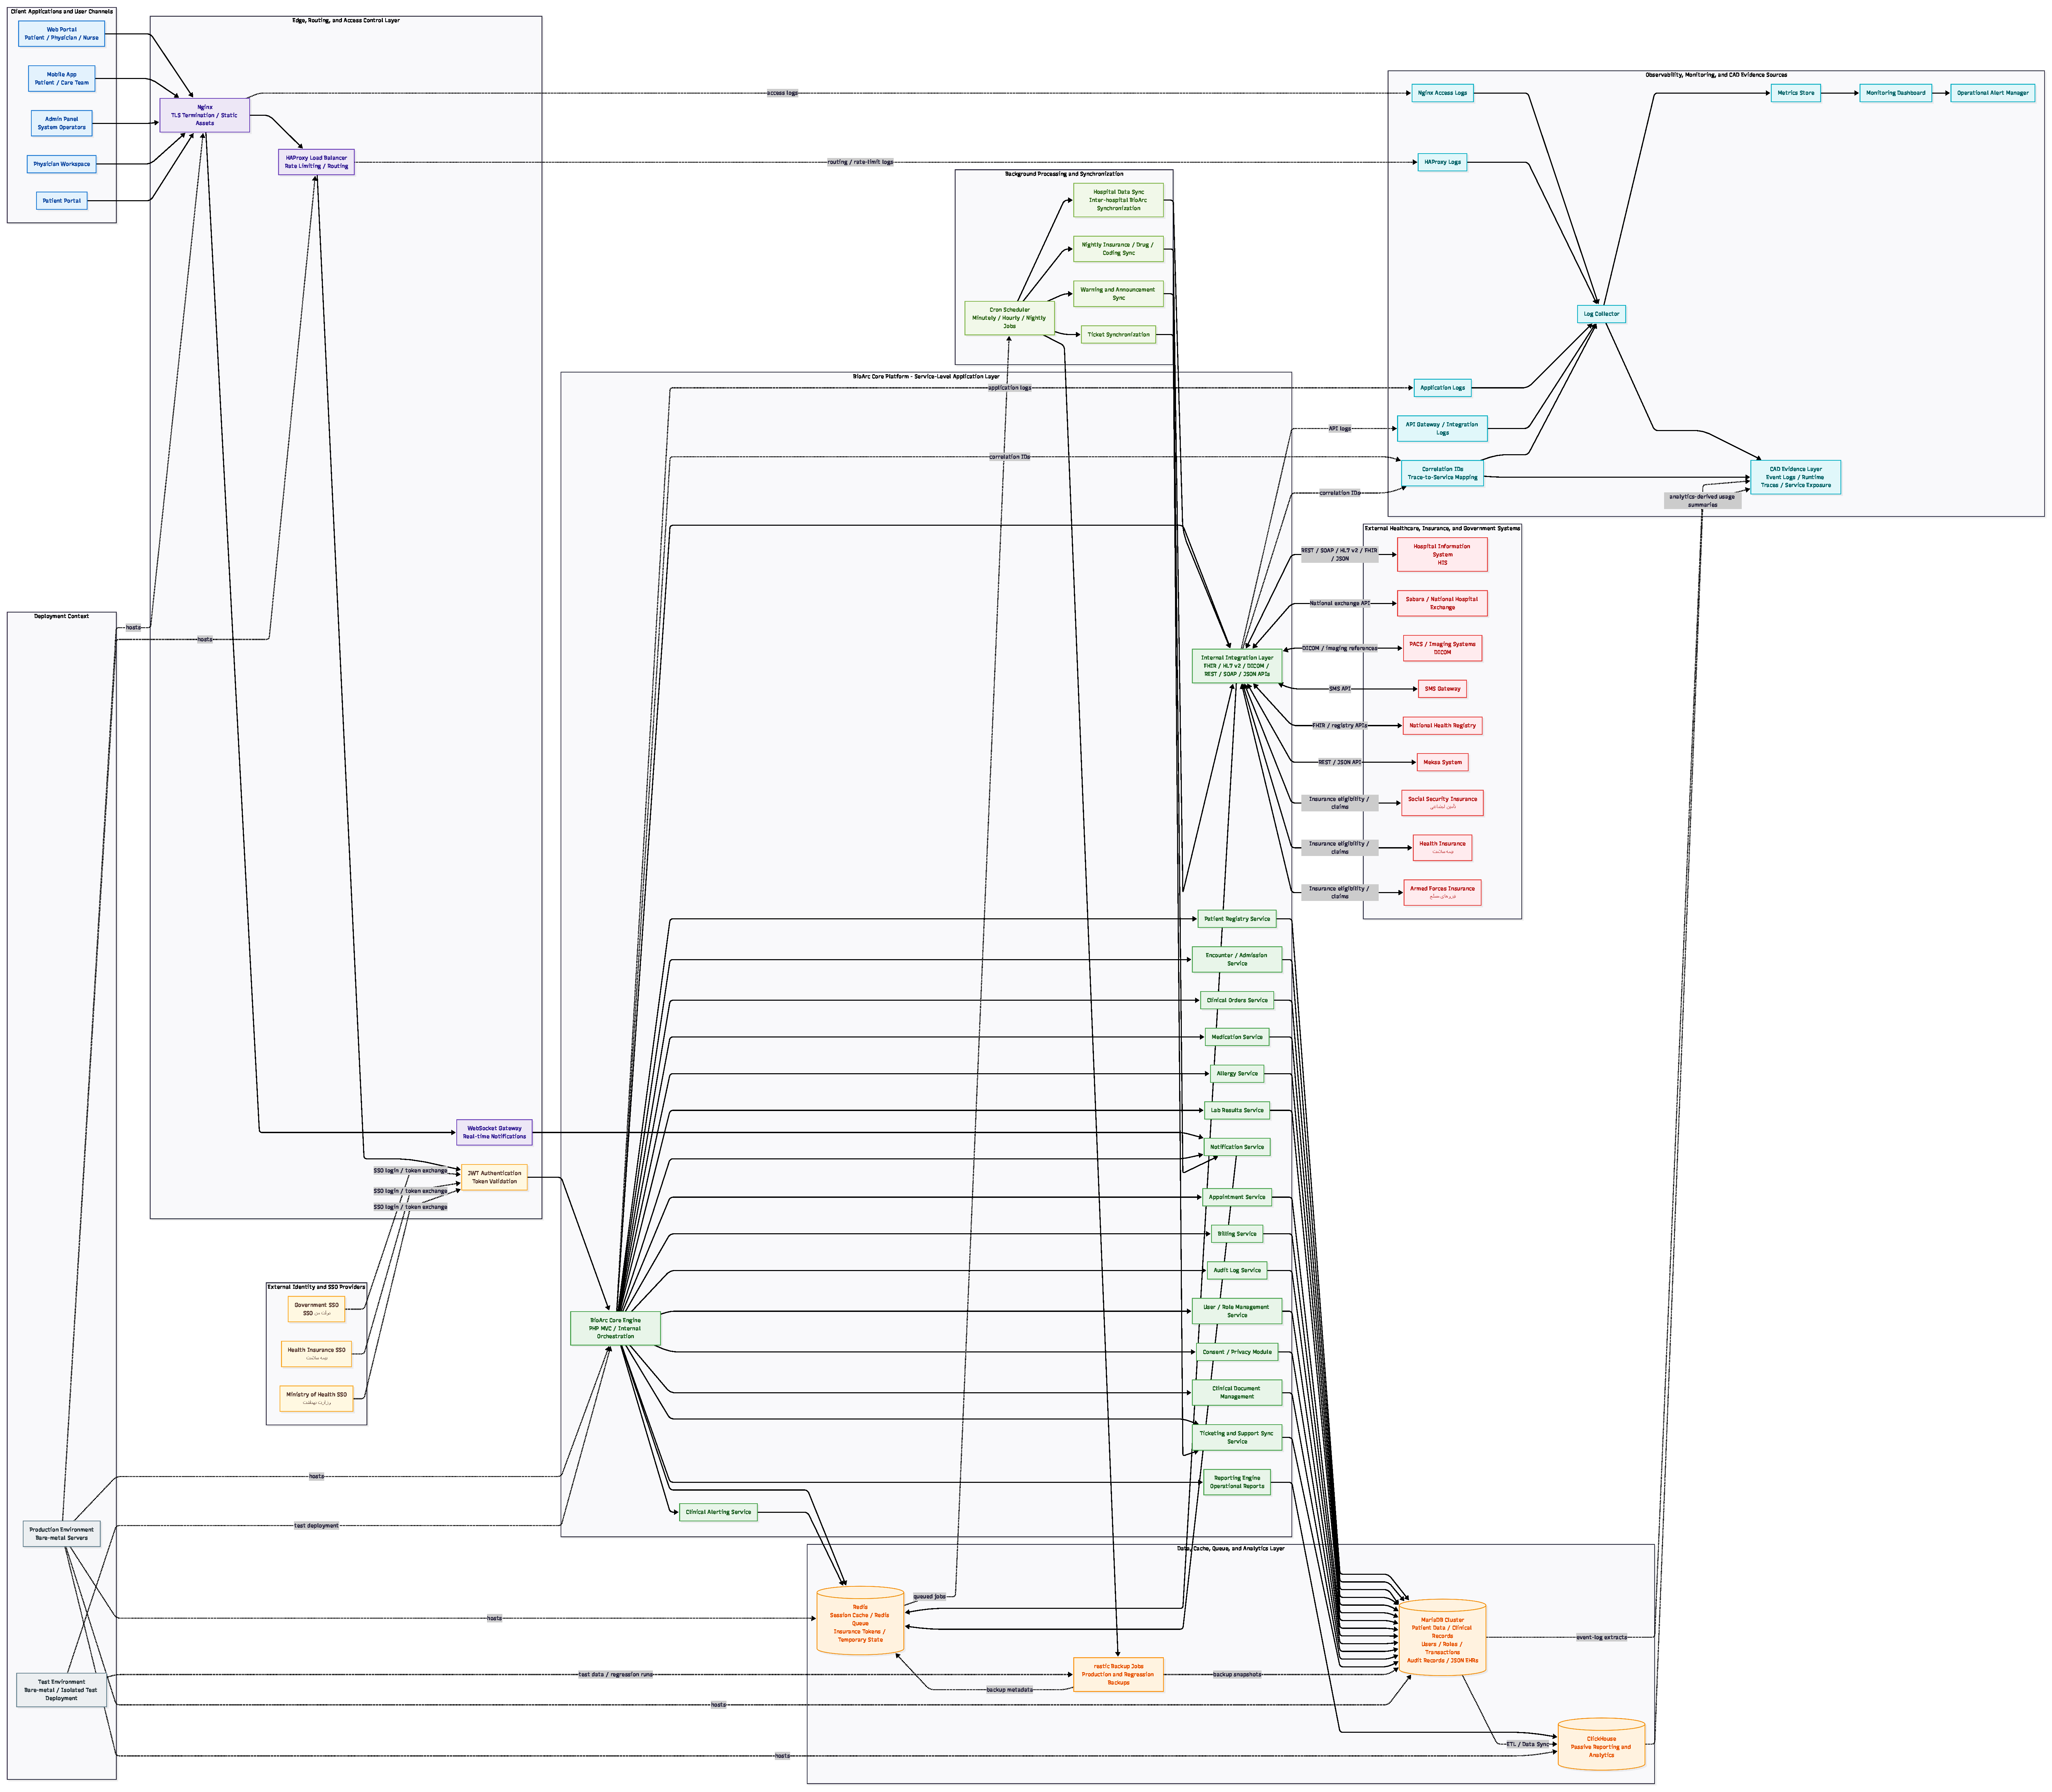
\includegraphics[width=\textwidth]{fig01_bioarc_overview.pdf}
\caption{A simplified service-level architecture and observability/data-flow view of the evaluated BioArc system.}
\label{fig:bioarc-overview}
\end{figure}

Figure~\ref{fig:cad-pipeline} summarizes the end-to-end analysis. Event logs are transformed into process variants and frequencies; clinical criticality is attached to those variants; distributed traces map observed activities to services; static and historical indicators produce component-fragility scores; and the combined evidence is used to rank components for engineering maintenance.

\begin{figure}[htbp]
\centering
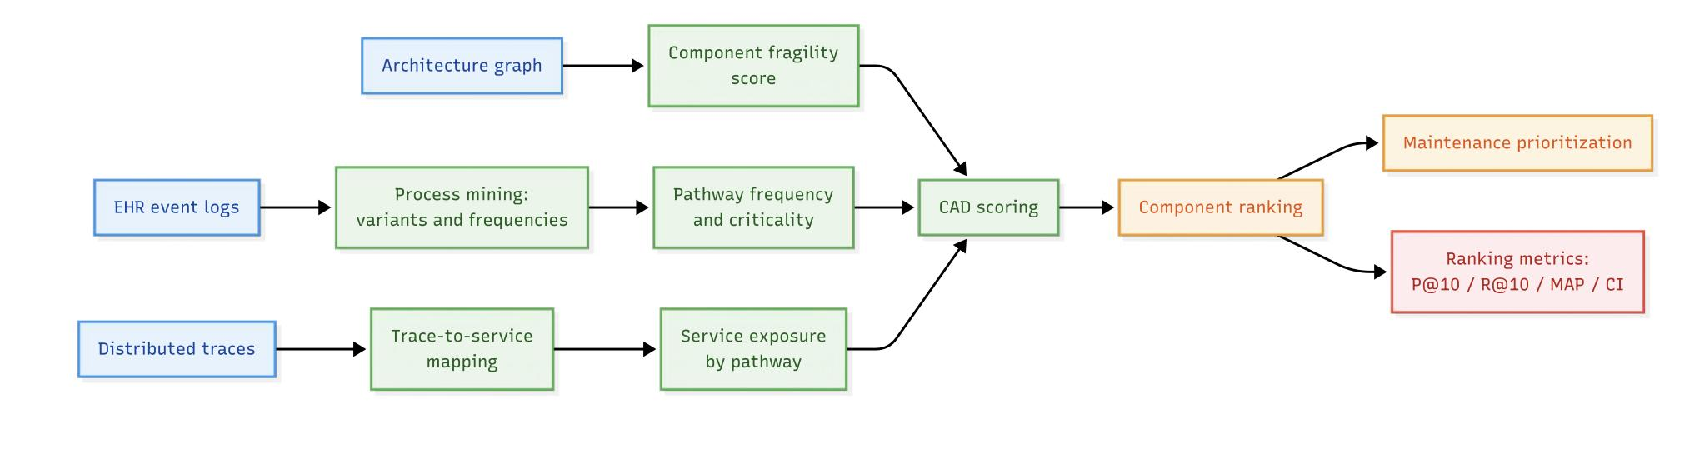
\includegraphics[width=\textwidth]{fig02_cad_pipeline.pdf}
\caption{The end-to-end \CAD analysis pipeline applied to the BioArc dataset.}
\label{fig:cad-pipeline}
\end{figure}

Table~\ref{tab:setup} summarizes the observation window, data volume, instrumentation coverage, process-discovery settings, and execution environment used in the evaluation.

\begin{table}[htbp]
\caption{BioArc evaluation setup.}
\label{tab:setup}
\small
\begin{tabularx}{\textwidth}{@{}p{0.43\textwidth}Y@{}}
\toprule
\textbf{Item} & \textbf{Value} \\
\midrule
Observation window & 12 months \\
Event-log activity records & 500,000 \\
Deployable services/components & 45 \\
Primary pathways & 14 \\
Clinical-informatics raters & 3 \\
Inter-rater agreement & Fleiss' $\kappa=0.82$ \\
Injected architecture-level defects & 120 \\
Components labeled relevant & 12 of 45 \\
Activities with complete trace mapping & 78.5\% \\
Cases with complete trace mapping & 64.1\% \\
Partially mapped activities & 15.2\% \\
Unmapped activities & 6.3\% \\
Process-discovery algorithm & Inductive Miner \\
Inductive Miner noise threshold & 0.8 \\
Rare-variant threshold & $<0.5\%$ of total frequency \\
Reference execution environment & Linux-4.4.0-x86\_64-with-glibc2.41; Python 3.13.5; 56 logical CPUs \\
Repeated evaluation runs & 30 (seeds 42--71) \\
Reference full-run wall-clock time & 6.13 s \\
Reference peak process memory & 582.51 MB \\
\bottomrule
\end{tabularx}
\end{table}

\subsection{Criticality elicitation and trace coverage}

Three clinical-informatics raters independently assigned each of the 14 primary pathways to one of the four bands in Table~\ref{tab:criticality}. Fleiss' $\kappa$ was computed from the independent ratings before discussion. The raters then reviewed disagreements and assigned the final band by consensus. Fleiss' $\kappa=0.82$ indicated high agreement. The final distribution comprised four low-, five moderate-, three high-, and two critical-pathway variants.

Trace quality was measured before scoring. Complete activity-level mapping was available for 78.5\% of activities, 15.2\% were partially mapped, and 6.3\% could not be reliably mapped. At case level, 64.1\% of cases had complete end-to-end mapping. These values are reported because incomplete instrumentation can systematically reduce the apparent exposure of a service and therefore depress its \CAD score.

\subsection{Injected-defect ground truth}

Injected defects served as controlled labels for architecture-relevant maintenance targets. The injection protocol and component selection were defined independently of the final \CAD scores. Each label linked a defect identifier to a service, defect category, affected pathways, criticality band, and related test identifiers. A component was labeled relevant when it contained at least one injected architecture-level defect. Across the 120 injected defects, 12 of the 45 components met this criterion. Table~\ref{tab:defects} summarizes the labeling protocol.

\begin{table}[htbp]
\caption{Injected-defect protocol used to construct controlled ground truth.}
\label{tab:defects}
\small
\begin{tabularx}{\textwidth}{@{}p{0.25\textwidth}Y@{}}
\toprule
\textbf{Element} & \textbf{Protocol} \\
\midrule
Defect target & Architecture- and service-level elements rather than arbitrary source lines. \\
Categories & Dependency misuse; unstable service interaction; schema/contract inconsistency; missing fallback; test-gap exposure; observability gap. \\
Selection & Components selected before \CAD ranking and independently of final scores. \\
Label construction & Defect ID, service ID, category, pathway exposure, criticality, and related test identifiers. \\
Relevance & A component is relevant if it contains at least one injected architecture-level defect. \\
\bottomrule
\end{tabularx}
\end{table}

\subsection{Baselines and evaluation measures}

Four methods were compared:
\begin{enumerate}
  \item \textbf{Static fragility}: ranks components using $F(C_j)$ only.
  \item \textbf{Frequency only}: ranks components according to observed pathway exposure without clinical criticality or structural fragility.
  \item \textbf{Unweighted process-aware}: combines structural fragility and trace-derived pathway exposure while treating all pathways as equally critical.
  \item \textbf{Full \CAD}: combines fragility, pathway frequency, clinical criticality, and trace-derived component exposure according to Eq.~\eqref{eq:cad}.
\end{enumerate}

For each run, precision at 10 (P@10) was the fraction of the first ten ranked components labeled relevant, and recall at 10 (R@10) was the fraction of all relevant components retrieved in the first ten positions. Average precision was computed over the complete 45-component ranking; MAP is the mean of average precision across the 30 runs. MRR is the mean reciprocal rank of the first relevant component. Table~\ref{tab:performance} reports means across runs. The bracketed intervals are 95\% bootstrap confidence intervals obtained using a run-level BCa bootstrap with 10,000 resamples. Cliff's $\delta$ compares full \CAD with each baseline; positive values favor full \CAD \cite{Efron1994Bootstrap,Cliff1993}.

\subsection{RQ1: Ranking effectiveness}

Table~\ref{tab:performance} reports the synthetic ranking results. Full \CAD achieved a mean P@10 of 0.93, R@10 of 0.77, MAP of 0.91, and MRR of 0.97 across the 30 runs. The best non-\CAD baseline, unweighted process-aware ranking, reached a mean P@10 of 0.65 and MAP of 0.59. Within the synthetic calibration, static fragility and frequency-only ranking performed less effectively than full \CAD.

\begin{table}[htbp]
\caption{Ranking effectiveness and runtime across 30 runs. Brackets report 95\% bootstrap confidence intervals for P@10, R@10, and MAP. Runtime is the mean method-specific scoring and ranking time for the 30-run synthetic workload on the reference environment.}
\label{tab:performance}
\small
\resizebox{\textwidth}{!}{%
\begin{tabular}{@{}lcccccc@{}}
\toprule
\textbf{Method} & \textbf{P@10} & \textbf{R@10} & \textbf{MAP} & \textbf{MRR} & \textbf{Runtime (s)} & \textbf{Cliff's $\delta$ (full \CAD vs.\ method)} \\
\midrule
Static fragility & 0.57 [0.54, 0.60] & 0.47 [0.45, 0.50] & 0.51 [0.47, 0.54] & 0.50 & 0.0020 & 1.00 (large) \\
Frequency only & 0.43 [0.38, 0.46] & 0.36 [0.32, 0.39] & 0.36 [0.33, 0.39] & 0.51 & 0.0023 & 1.00 (large) \\
Unweighted process-aware & 0.65 [0.60, 0.69] & 0.54 [0.50, 0.57] & 0.59 [0.55, 0.63] & 0.63 & 0.0021 & 0.98 (large) \\
Full \CAD & 0.93 [0.88, 0.95] & 0.77 [0.74, 0.79] & 0.91 [0.88, 0.93] & 0.97 & 0.0020 & Reference \\
\bottomrule
\end{tabular}}
\end{table}


\subsection{RQ2: Marginal contribution of clinical criticality}

Removing clinical criticality reduced mean P@10 from 0.93 to 0.65 and MAP from 0.91 to 0.59 (Table~\ref{tab:ablation}). This comparison isolates the contribution of $K(P_i)$ beyond structural fragility and observed execution frequency. Without criticality, common but lower-risk workflows receive the same process weight as safety-sensitive pathways. Removing fragility or trace exposure also reduced the reported ranking measures, indicating that the observed full-\CAD performance depended on the combination of the four evidence sources.

In Table~\ref{tab:ablation}, top-10 stability denotes the mean value of $|T_{10}^{(a)}\cap T_{10}^{(\mathrm{full})}|/10$ across the 30 runs.

\begin{table}[htbp]
\caption{Mean ablation results across 30 evaluation runs.}
\label{tab:ablation}
\small
\begin{tabularx}{\textwidth}{@{}Ycccc@{}}
\toprule
\textbf{Configuration} & \textbf{P@10} & \textbf{R@10} & \textbf{MAP} & \textbf{Top-10 stability} \\
\midrule
Full \CAD & 0.93 & 0.77 & 0.91 & 1.00 \\
Without criticality & 0.65 & 0.54 & 0.59 & 0.61 \\
Without frequency & 0.83 & 0.69 & 0.87 & 0.71 \\
Without fragility & 0.62 & 0.52 & 0.67 & 0.67 \\
Without trace exposure & 0.57 & 0.47 & 0.51 & 0.43 \\
\bottomrule
\end{tabularx}
\end{table}

\subsection{RQ3: Robustness and sensitivity}

Table~\ref{tab:sensitivity} reports sensitivity to five pre-specified perturbations. Uniform fragility weighting replaced the baseline vector $(0.20,0.15,0.25,0.20,0.20)$ with $(0.2,0.2,0.2,0.2,0.2)$. The alternative criticality mapping replaced $(0.25,0.50,0.75,1.00)$ with $(0.10,0.40,0.70,1.00)$. The frequency perturbation increased the rare-variant threshold from 0.5\% to 1.0\%. Trace completeness was reduced or increased by 20\% using a procedure that uniformly dropped 20\% of observed nonzero trace links for the reduced-coverage condition and recovered 20\% of missing links from the known synthetic pathway--component map for the increased-coverage condition. Spearman's $\rho$ and Kendall's $\tau$ were computed over the complete 45-component rankings, and top-10 overlap was computed relative to the unperturbed full-\CAD ranking.

Under these perturbations, uniform fragility weights preserved a mean of 9.9 of the ten top-ranked components and yielded Spearman's $\rho=0.998$. Alternative criticality mapping preserved 8.8 of ten and yielded $\rho=0.974$. Reducing trace completeness by 20\% produced the largest observed shift, preserving 7.7 top-10 components with $\rho=0.868$. These synthetic results identify trace completeness as the strongest examined perturbation.

\begin{table}[htbp]
\caption{Sensitivity of the \CAD ranking relative to the unperturbed full-\CAD configuration.}
\label{tab:sensitivity}
\small
\begin{tabularx}{\textwidth}{@{}Yccc@{}}
\toprule
\textbf{Perturbation} & \textbf{Top-10 overlap} & \textbf{Spearman $\rho$} & \textbf{Kendall $\tau$} \\
\midrule
Uniform fragility weights & 9.9/10 & 0.998 & 0.980 \\
Alternative criticality mapping & 8.8/10 & 0.974 & 0.882 \\
Frequency threshold 1.0\% & 9.9/10 & 0.999 & 0.993 \\
Trace completeness reduced by 20\% & 7.7/10 & 0.868 & 0.764 \\
Trace completeness increased by 20\% & 9.9/10 & 0.988 & 0.978 \\
\bottomrule
\end{tabularx}
\end{table}

\subsection{RQ4: Runtime overhead}

On the committed reference run, the complete synthetic experiment, including 30 runs, BCa confidence intervals, result serialization, and figure generation, required 6.13 seconds and reached a peak process memory of 582.51 MB. Method-specific scoring and ranking over the 30-run workload required 0.0020, 0.0023, 0.0021, and 0.0020 seconds for static fragility, frequency-only, unweighted process-aware, and full \CAD, respectively. Timing included pathway-frequency resampling, trace-state resampling, exposure aggregation, fragility normalization, \CAD scoring, and ranking, and excluded database extraction, log transfer, one-time environment initialization, manuscript compilation, and figure generation from the method-specific measurements. Runtime values are environment-dependent.

\section{Discussion}\label{sec:discussion}

\subsection{Why process-aware ranking changes maintenance priorities}

The principal result is not that structural debt metrics are unhelpful; it is that they are incomplete when the same architecture supports workflows with substantially different clinical consequences. Static fragility identified components that were difficult to maintain, but it could not distinguish whether those components mediated a high-criticality medication or alerting pathway, a routine documentation pathway, or a low-frequency archival function. Frequency-only ranking captured operational exposure but systematically favored common activity. Full \CAD elevated components that were simultaneously fragile, observed in runtime traces, and exposed to pathways rated as clinically important.

\subsection{The role of criticality weighting}

The ablation results indicate that criticality weighting contributed materially to ranking effectiveness. Removing $K(P_i)$ reduced both retrieval quality and top-10 stability. This finding supports the methodological premise of the paper: in a safety-relevant system, engineering priority should reflect not only how often a pathway is executed but also what type of clinical work the pathway supports. Nevertheless, criticality scores are expert judgments rather than direct measurements of harm. They should be treated as governed, reviewable inputs and subjected to sensitivity analysis rather than embedded as opaque constants.

\subsection{Implications for engineering practice}

A practical \CAD workflow could be integrated into periodic architecture governance. Engineering teams can recompute rankings after major releases, service splits, schema changes, instrumentation improvements, or incident reviews. The ranked list can inform refactoring backlog order, architecture-review depth, integration-test allocation, observability work, and targeted failure-injection exercises. The method is most useful when each recommendation remains traceable to its contributing evidence: fragility indicators, pathway frequencies, criticality bands, and runtime traces.

\subsection{Interpretive limits}

\CAD is an engineering prioritization method. It does not establish that a component is unsafe, predict patient harm, replace clinical hazard analysis, or certify regulatory compliance. The controlled injected-defect labels measure ranking performance under the case-study protocol. Prospective evidence would be required to show that applying \CAD reduces production incidents, improves clinical outcomes, or changes patient-safety risk.

\section{Threats to Validity}\label{sec:threats}

\subsection{Construct validity}

Structural fragility is a composite of normalized software indicators and therefore depends on the operational definitions and weights selected. Clinical criticality is an expert-assessed construct that may vary across institutions and local workflows. Trace-derived exposure can be underestimated for weakly instrumented services. Finally, injected defects are a controlled proxy for architecture-relevant components rather than a complete representation of naturally occurring production failures.

\subsection{Internal validity}

The scoring configuration was fixed before the injected-defect labels were used for assessment, reducing the risk of post-hoc parameter tuning. Even so, the defect-injection process may favor categories that are easier to express or observe. The independence of component selection from final scores, the documented label schema, repeated runs, ablations, and sensitivity analysis mitigate but do not eliminate this threat.

\subsection{External validity}

The simulation represents one BioArc-like synthetic architecture with 45 deployable components and 14 primary pathways; it does not reproduce the full heterogeneity of a production institutional environment. Architecture styles, trace quality, workflow semantics, and clinical-risk rubrics differ across hospitals and vendors. Replication is therefore needed in other EHR systems, integration architectures, and healthcare domains before broad generalization.

\subsection{Conclusion validity}

Thirty repeated runs and BCa bootstrap confidence intervals characterize synthetic run-to-run uncertainty, but the calibration ranks only 45 generated components and cannot establish external validity for production EHR systems. The effect-size comparisons and retrieval metrics should be interpreted in combination rather than as isolated proof. The sensitivity analysis demonstrates ranking consistency under the examined perturbations, not robustness to every possible scoring or missing-data mechanism.

\subsection{Privacy and governance}

Operational event logs and distributed traces may contain sensitive clinical or operational metadata even after de-identification. Replication packages should therefore separate shareable schemas, synthetic data, and scoring code from restricted raw logs and traces. Any reuse must follow local governance and data-protection requirements.

\section{Replication Materials}\label{sec:replication}

The shareable replication package contains the event schema, preprocessing logic, trace-linking rules, \CAD computation code, plotting scripts, random seeds, software-version metadata, and a synthetic dataset preserving the structural properties needed to execute the pipeline. The package is available at \url{https://github.com/tanhaei/CAD}. Raw operational logs and distributed traces are excluded because they may retain sensitive clinical or operational metadata after de-identification.

\section{Conclusion}\label{sec:conclusion}

This paper introduced Clinical-Architectural Debt, a process-aware metric for prioritizing maintenance in distributed EHR systems. The method combines component fragility, observed pathway frequency, expert-assessed clinical criticality, and trace-derived service exposure. In the simulation-only calibration, full \CAD ranked generated components containing injected architecture-level defects more effectively than static-fragility, frequency-only, and unweighted process-aware baselines. Ablation analysis indicated that criticality, frequency, fragility, and trace exposure each contributed to ranking performance, while sensitivity analysis showed substantial stability under alternative assumptions. The synthetic evidence demonstrates executable internal consistency of the proposed pipeline; it does not establish empirical effectiveness or clinical safety impact in a production setting. Future work should replicate the method across organizations, use natural incident and postmortem labels where governance permits, model uncertainty in criticality and trace completeness explicitly, and evaluate whether \CAD-guided maintenance improves long-term architecture outcomes.

\section*{CRediT authorship contribution statement}

\textbf{Mohammad Tanhaei:} Conceptualization, Data curation, Formal analysis, Methodology, Project administration, Resources, Software, Supervision, Validation, Visualization, Writing -- original draft, Writing -- review and editing.

\section*{Funding}

This research received no specific grant from any funding agency in the public, commercial, or not-for-profit sectors.

\section*{Declaration of competing interest}

The author declares no known competing financial interests or personal relationships that could have appeared to influence the work reported in this paper.

\section*{Ethics and governance}

The external validation analyses were conducted on de-identified retrospective records obtained under institutional data-governance procedures. According to the determination of the Ilam University Ethics Committee, the requirement for individual informed consent was waived for this retrospective analysis.

\section*{Data availability}

Raw operational event logs and distributed traces are not publicly available because of governance and confidentiality restrictions. The synthetic dataset, schemas, analysis code, and figure-generation scripts are available at \url{https://github.com/tanhaei/CAD}.

\appendix
\setcounter{figure}{0}
\renewcommand{\thefigure}{A.\arabic{figure}}
\section{BioArc Detailed Architecture}\label{app:architecture}

Figures~\ref{fig:appendix-service} and~\ref{fig:appendix-observability} provide the detailed architecture views used to contextualize the BioArc case study. Figure~\ref{fig:appendix-service} focuses on the service-level application architecture and external healthcare integrations, while Figure~\ref{fig:appendix-observability} focuses on observability, synchronization, \CAD evidence inputs, backup, and isolated test-support flows.

\begin{sidewaysfigure}
\centering
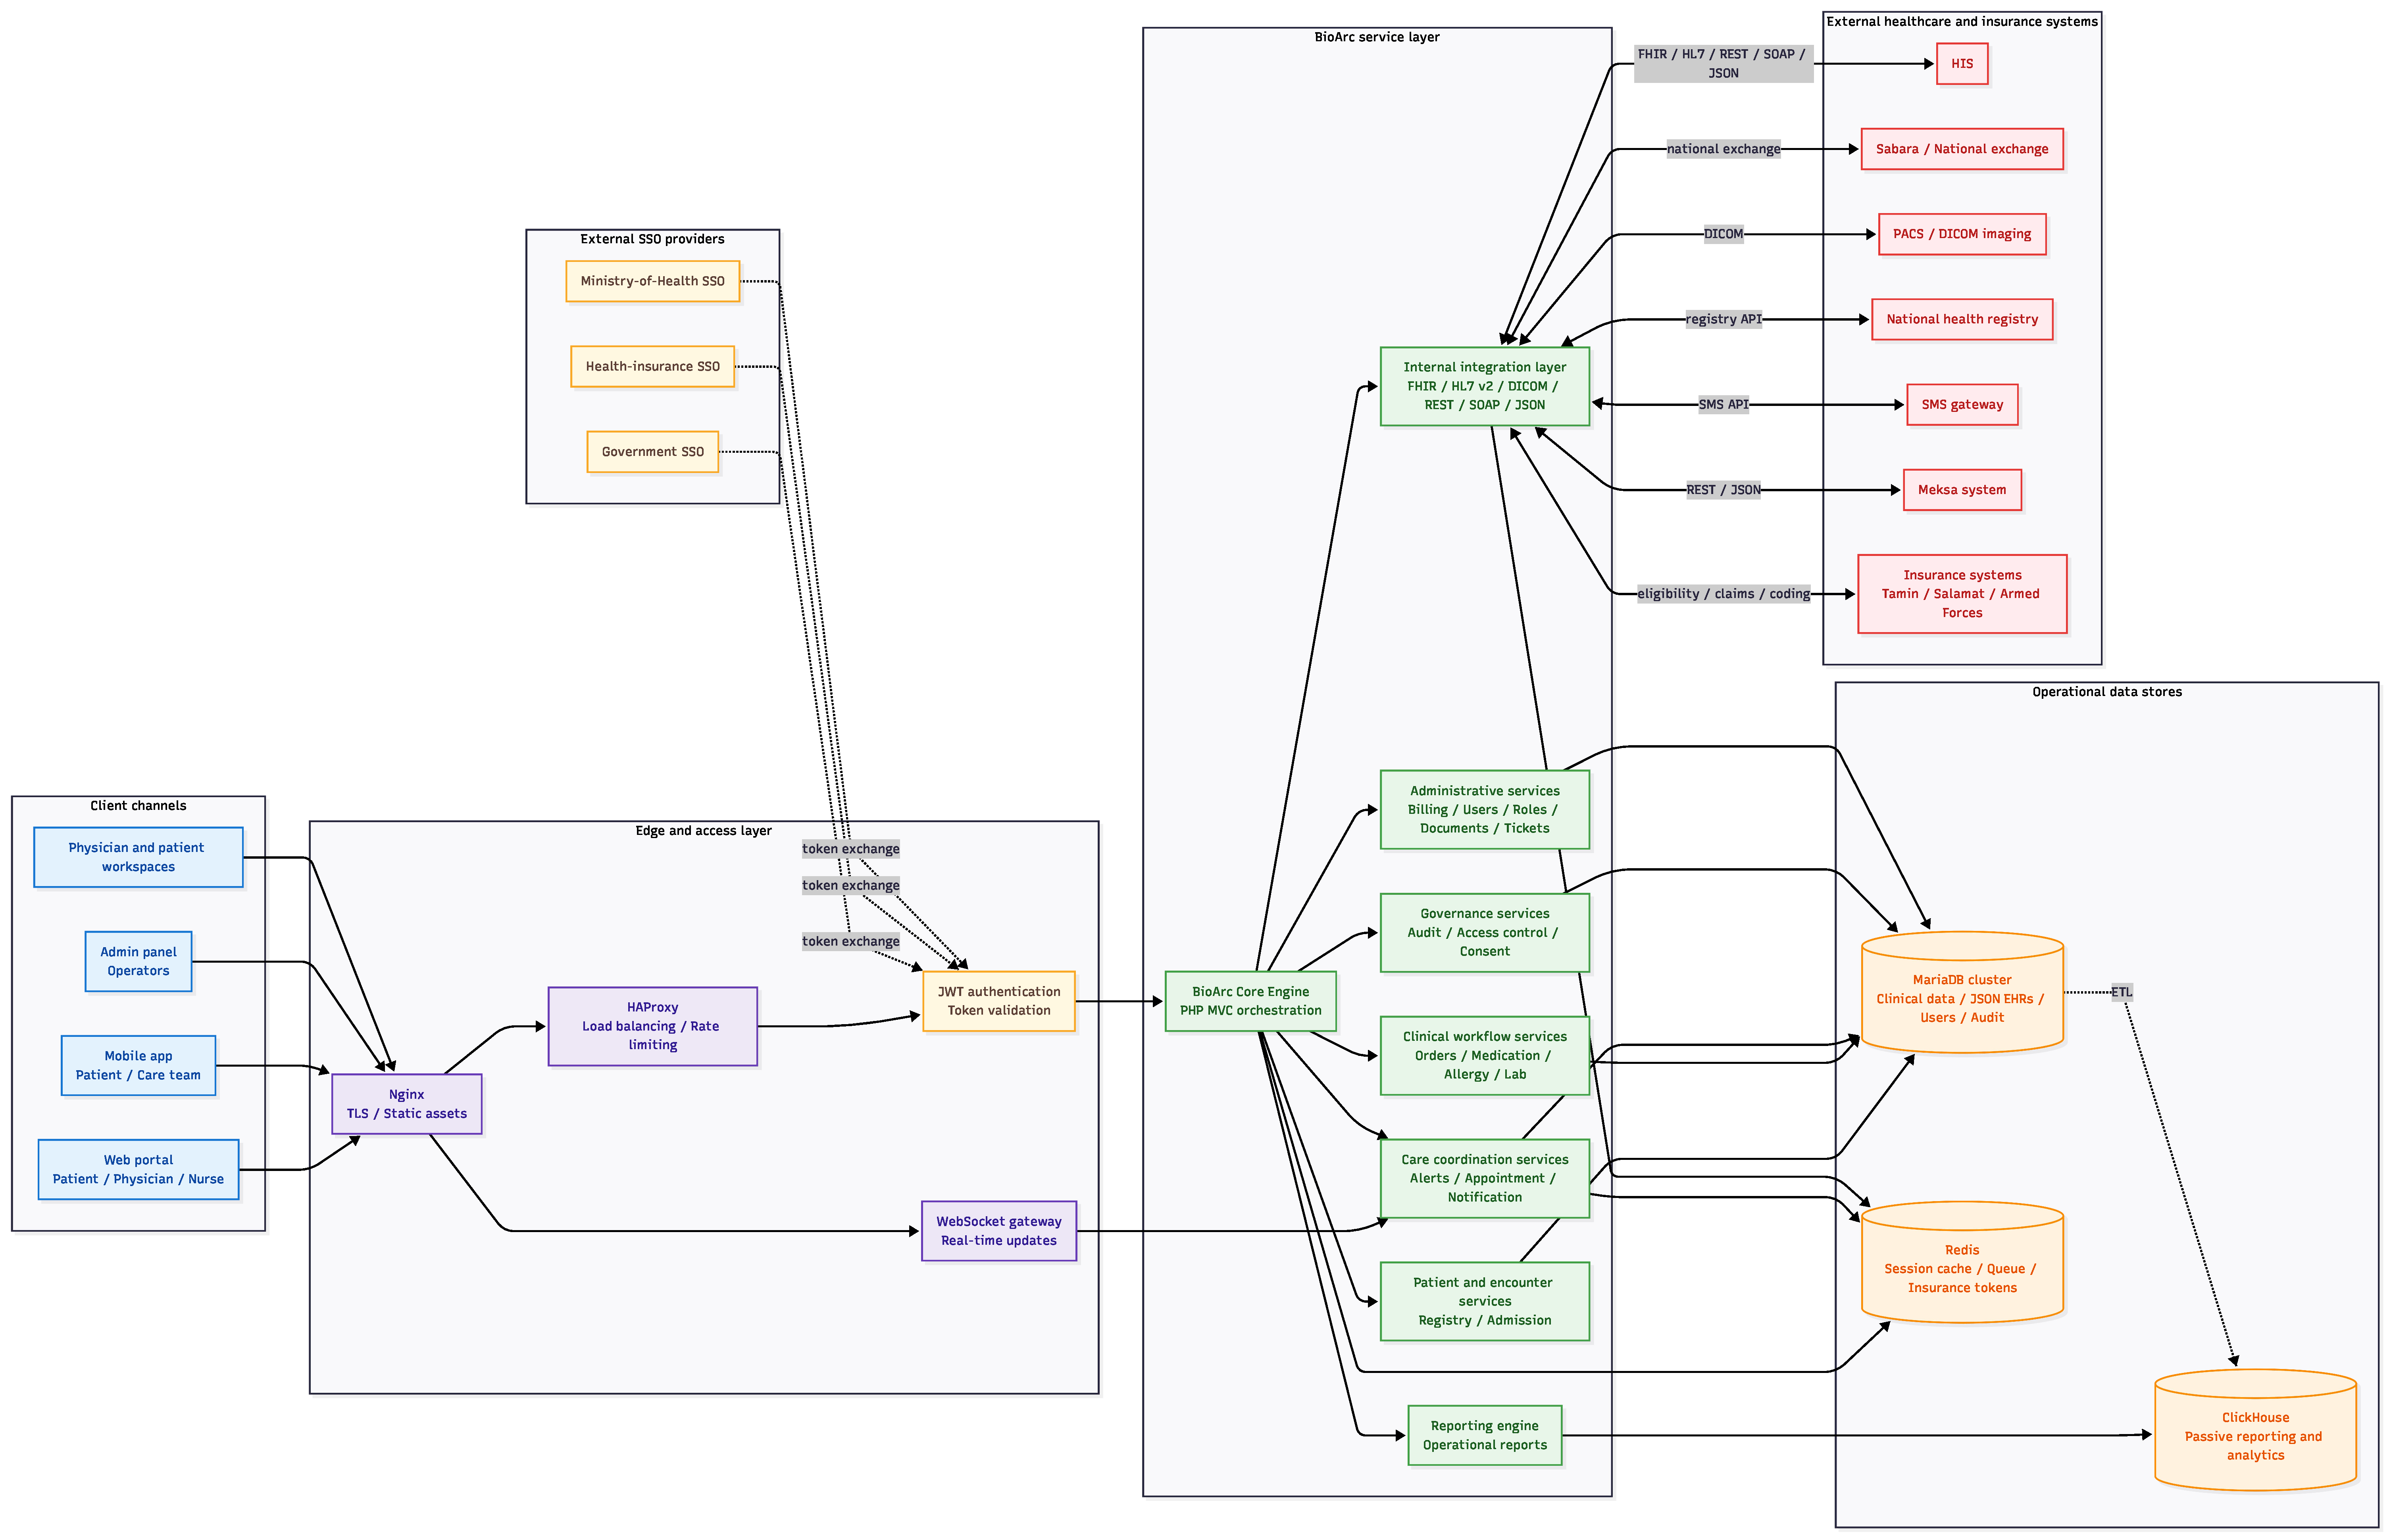
\includegraphics[width=\textheight]{bioarc_service_external.pdf}
\caption{Detailed BioArc service-level architecture and external integrations. The diagram shows client channels, edge routing, authentication, external SSO providers, the BioArc core service layer, operational data stores, and integrations with external healthcare, insurance, imaging, messaging, and national-registry systems.}
\label{fig:appendix-service}
\end{sidewaysfigure}

\begin{sidewaysfigure}
\centering
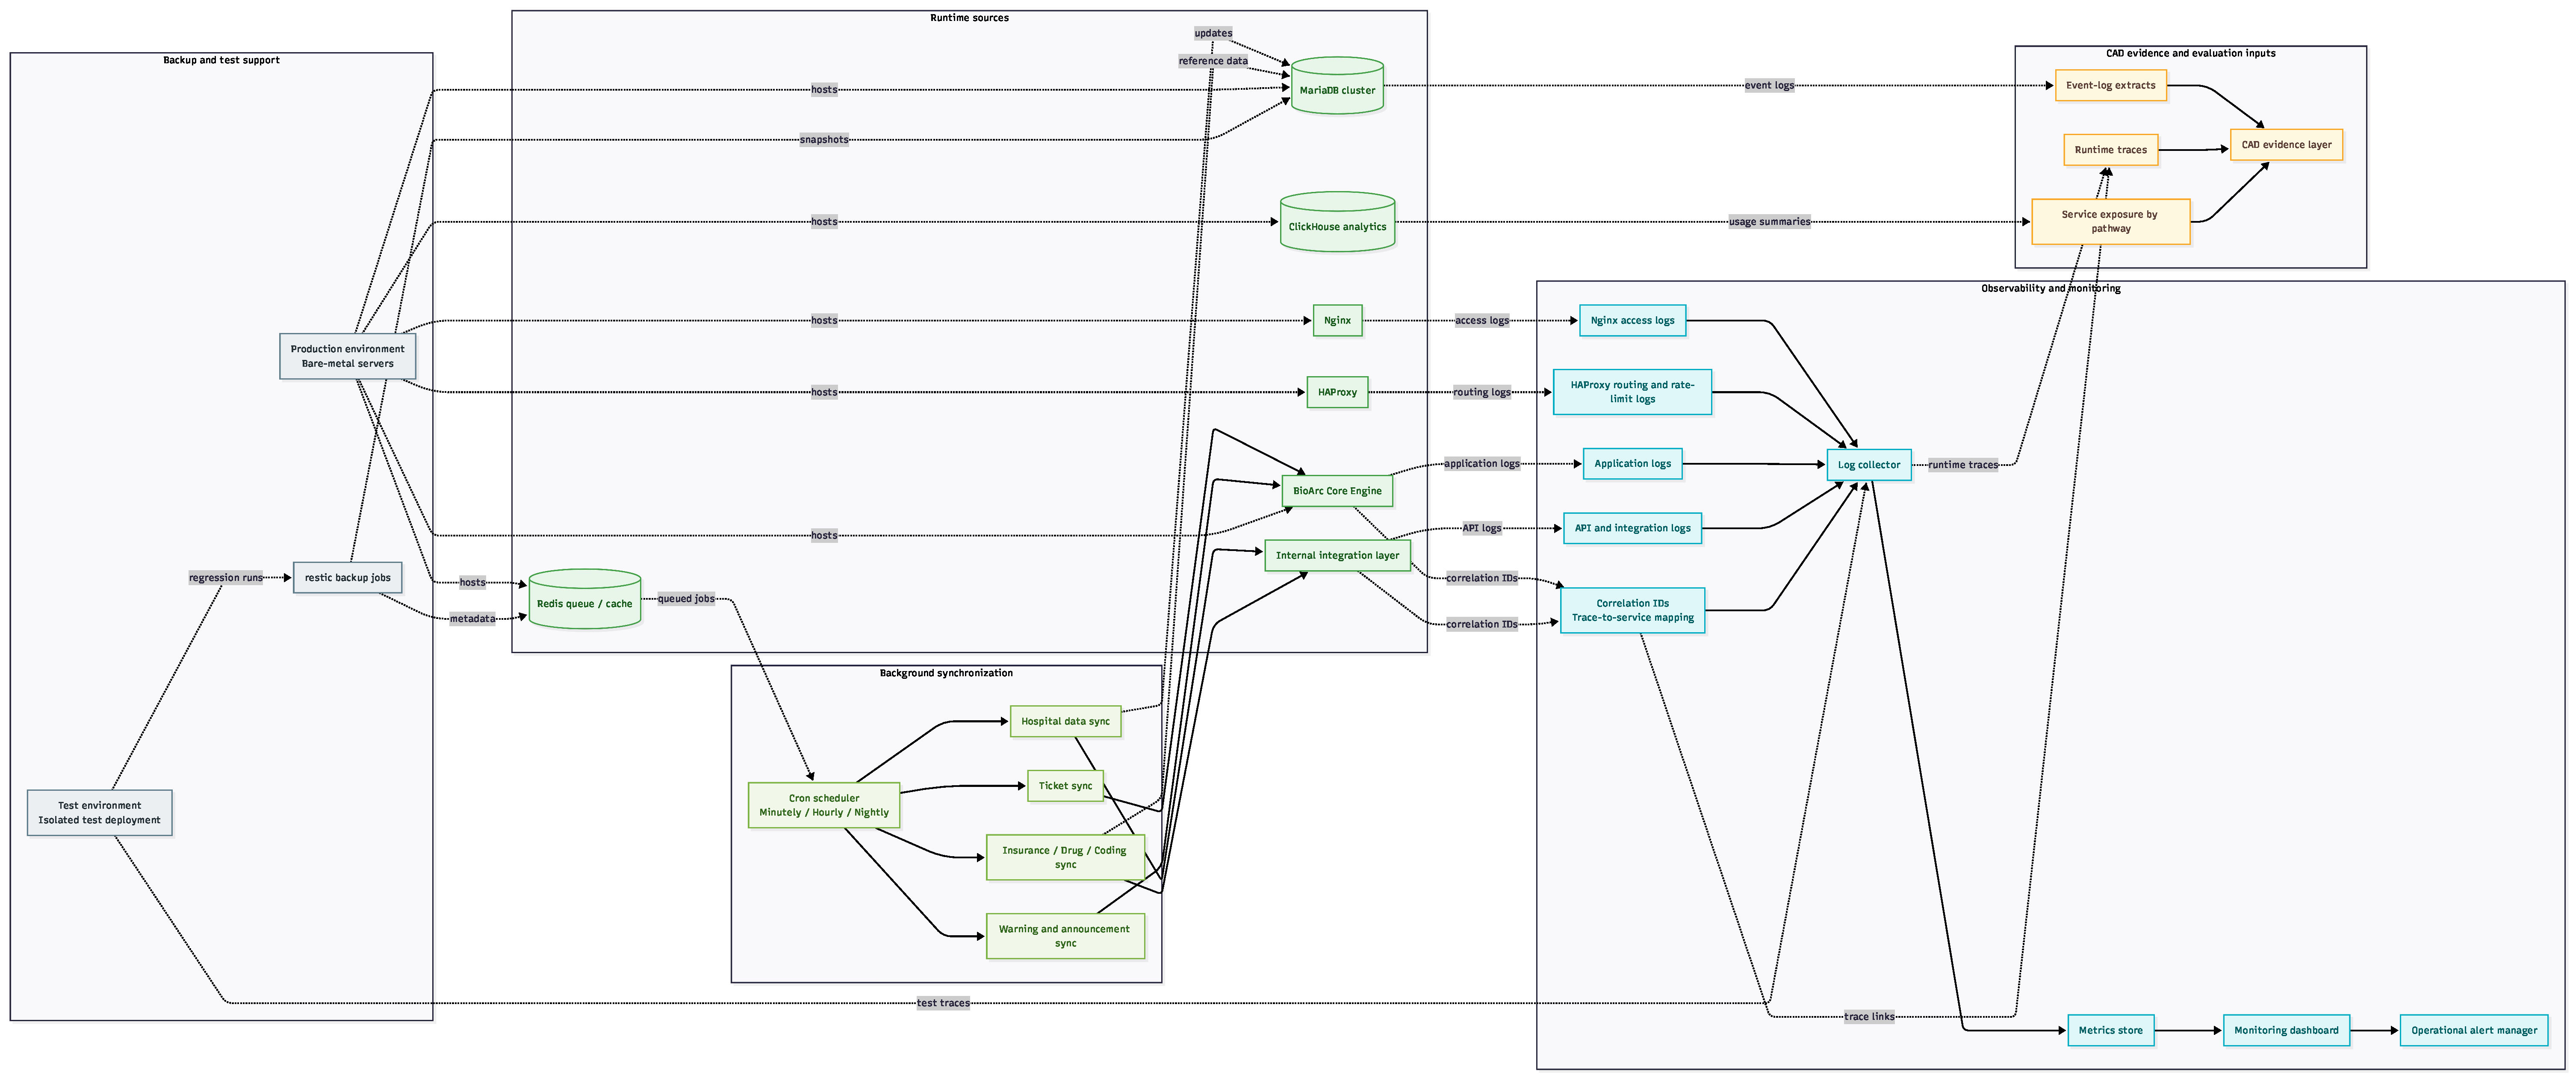
\includegraphics[width=\textheight]{bioarc_observability_sync.pdf}
\caption{BioArc runtime observability, background synchronization, \CAD evidence, backup, and isolated test-support data flows.}
\label{fig:appendix-observability}
\end{sidewaysfigure}

\bibliographystyle{elsarticle-num}
\bibliography{references}

\end{document}
